\section{Prologo nel XIX secolo}
La nascita della teoria degli insiemi è una storia complicata di cui so pochissimo. Però, persone che ne sanno molto più di me hanno sostenuto l'opinione che il problema seguente
abbia avuto un ruolo. Come che sia, è almeno un'introduzione possibile.

\begin{problem}
Data una serie trigonometrica:
\[ S(x) = c_0 + \sum_{i=1}^{+\infty}a_i\sin{(ix)}+b_i\cos{(ix)}
	\]
se, per ogni $x \in \RR$, sappiamo che $S(x)$ converge a 0, possiamo dire che i coefficienti $c_0,a_i,b_i$ sono tutti 0?
\end{problem}

Risolto positivamente da \href{https://it.wikipedia.org/wiki/Georg_Cantor}{\textcolor{purple}{Georg Cantor}} nel 1870.

\begin{definition}
Diciamo che $X \subseteq \RR$ è un \vocab{insieme di unicità} se, per ogni serie trigonometrica:
\[ S(x) = c_0 + \sum_{i=1}^{+\infty}a_i\sin{(ix)}+b_i\cos{(ix)}
	\]
vale la seguente implicazione:
\[ \text{$S(x)$ converge a 0 per tutti gli $x\not\in X$} \implies \text{tutti i coefficienti $c_0,a_i,b_i$ sono nulli}
	\]
\end{definition}

\begin{example}
	Per il risultato di Cantor, $\emptyset$ è di unicità.
\end{example}

\begin{problem}
	Quali sottoinsiemi di $\RR$ sono di unicità?
\end{problem}

\begin{fact}[Criterio per gli insiemi di unicità]
Dato $X \subseteq \RR$ se (ma non solo se) \textcolor{purple}{ogni funzione continua $f : \RR \to \RR$ che soddisfi:
\begin{itemize}
	\item per ogni intervallo aperto $\left]a,b\right[$ con $]a,b[ \,\cap\, X = \emptyset$, $f_{| \, ]a,b[}$ è lineare.
	\item per ogni $x \in \RR$, se $f$ ha derivate destre e sinistre in $x$, allora queste coincidono\footnote{Ovvero $f$ non ha punti angolosi.}.
\end{itemize}
è lineare}\footnote{$f(x) = \alpha x + \beta$.}, allora $X$ è di unicità.
\end{fact}

\textcolor{MidnightBlue}{D'ora in avanti diremo che un insieme rispetta le ipotesi criterio, o ha la proprietà $(\star)$, se soddisfa il fatto in \textcolor{purple}{viola}, e quindi è di unicità per il fatto sopra.}

\begin{example}
	$X = \{\ldots,a_{-2},a_{-1},a_0,a_1,a_2,\ldots\} = \{a_i | i \in \ZZ\}$ con $\ldots < a_{-2} < a_{-1} < a_0 < a_1 < a_2 <\ldots$, $\lim_{i \to +\infty} a_i = +\infty$, $\lim_{i \to -\infty} a_i = -\infty$ ha la 
	proprietà data dal \hyperref[unicità]{Fatto 1.5}, quindi è di unicità.
\end{example}

\begin{notexample}
L'intervallo $[0,1]$ o $\RR$ non hanno la proprietà espressa dall'\hyperref[unicità]{Fatto 1.5}.
\end{notexample}

\begin{notexampleb}
Per l'\vocab{insieme di Cantor} non vale il \hyperref[unicità]{Fatto 1.5}.
\end{notexampleb}

Possiamo costruire l'insieme di Cantor a partire dall'intervallo $C_0 = [0,1]$ nel seguente modo:

\begin{figure}[H]
	\centering
	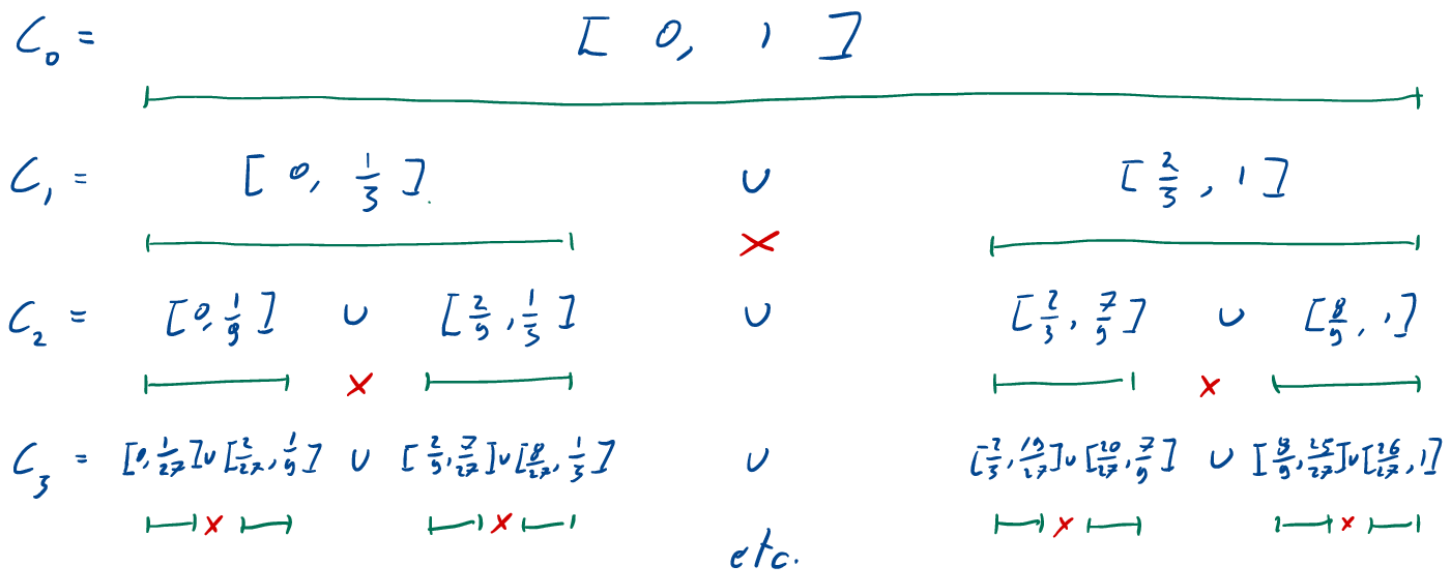
\includegraphics[width=12.5cm]{immagini/cantor.png}
\end{figure}

ovvero, preso l'intervallo $[0,1]$ possiamo dividerlo in tre parti e rimuovere la parte centrale $\left]\frac 13, \frac 23\right[$, chiamiamo gli intervalli rimanenti $C_1$, possiamo iterare il procedimento sui due segmenti di $C_1$ ed ottenere $C_2,C_3,\ldots, C_{n+1} = \frac{C_n}{3} \cup \left(\frac{C_n}{3} + \frac{2}{3}\right),\ldots$, a questo punto 
definiamo l'insieme di Cantor $C$ come:
\[ C := \bigcap_{i \in \NN}C_i
	\]
Esiste una funzione continua (e debolmente crescente) $f : \RR \to \RR$ detta \vocab{scala di Cantor} (o \vocab{scala del diavolo}), tale che $f^{\prime}(x) = 0$ per $x \not\in C$ e non è 
derivabile in $x \in C$.

\begin{figure}[H]
	\centering
	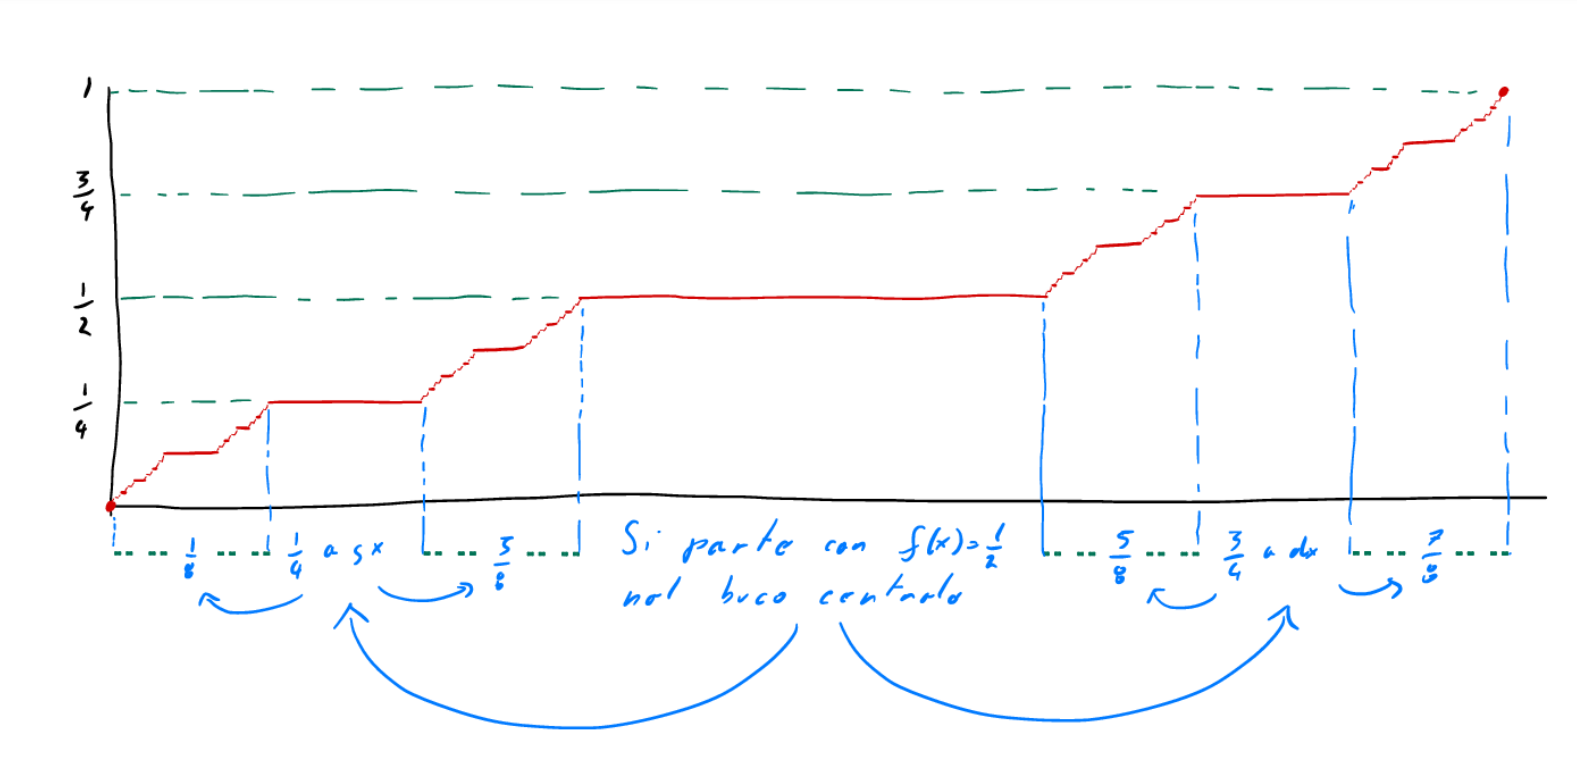
\includegraphics[width=13.5cm]{immagini/scalacantor.png}
\end{figure}

tale funzione si costruisce aggiungendo tratti costanti (prima $\frac 12$, poi $\frac 14$, $\frac 34$ e così via, dividendo l'intervallo $[0,1]$ sull'asse delle ordinate in parti uguali) alle parti eliminate sull'intervallo
$[0,1]$ sull'asse delle ascisse per costruire l'insieme di Cantor.

\begin{note}
Per $\QQ$ e $C$ non vale il \hyperref[unicità]{Fatto 1.5} ma, in realtà, sono di unicità.
\end{note}

\begin{exampleb}[$a_n \uparrow l$]
L'insieme degli elementi di una successione crescente col suo limite è un esempio di insieme di unicità.
\end{exampleb}

\begin{figure}[H]
	\centering
	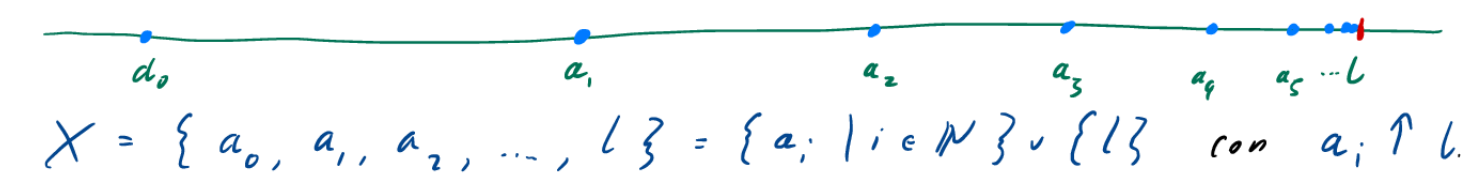
\includegraphics[scale=0.35]{immagini/succunic.png}
\end{figure}

Dimostriamo quindi che $X$ è un insieme di unicità.
\begin{proof}
Per ipotesi la funzione $f$ è lineare in $]-\infty, a_0[$ , $]a_0,a_1[$ , $]a_1,a_2[$ , $\ldots$ quindi nei punti $a_0,a_1,a_2,\ldots$ ammette ovviamente derivata destra e sinistra. 
Siccome, sempre per ipotesi, $f$ è continua e non ammette punti angolosi, questi punti non possono essere angolosi, per cui $f_{-}'(a_i) = f_{+}'(a_i)$, ovvero le rette $f_{|\,]-\infty, a_0[}$, $f_{|\,]a_0,a_1[}$, etc. hanno lo stesso coefficiente angolare.
Pertanto, per continuità, $f_{|\,]-\infty, l[}$ è lineare e per ipotesi lo è anche $f_{|\,]l,+\infty[}$, quindi $f$ è lineare.
\end{proof}

\begin{examplebb}[Successione di successioni crescenti]
L'insieme degli elementi di una successione crescente di successioni crescenti è un insieme di unicità.
\end{examplebb}

	\begin{figure}[H]
		\centering
		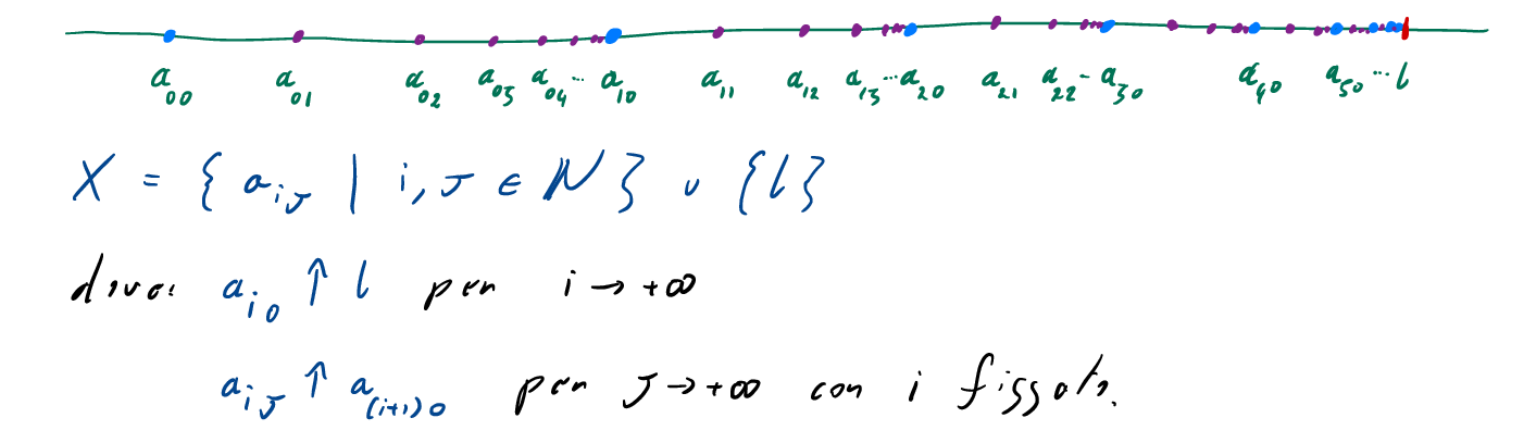
\includegraphics[width=12.5cm]{immagini/succunic2.png}
	\end{figure}

Dimostriamo che $X$ è di unicità.
\begin{proof}
In ciascuno degli intervalli $]a_{i0}, a_{(i+1)0}[$, $f$ è lineare, ragionando come nell'esempio precedente, ci siamo ridotti alla situazione
- di nuovo - dell'esempio precedente con $a_i^{\prime} = a_{i0}$.
\end{proof}

\subsection{Digressione: insiemi numerabili}
\begin{definition}
	Un insieme $X$ è \vocab{numerabile} se è il supporto di una successione, $X = \{a_0,a_1,a_2,\ldots\} = \{a_i | i \in \NN\}$, con $a_i \ne a_j$ per ogni $i \ne j$.\footnote{O in altre parole se esiste $f : \NN \to X$ biunivoca.}
\end{definition}

\begin{example}
	Alcuni esempi di insiemi numerabili sono:
	\begin{itemize}
		\item $\NN$, l'insieme dei numeri naturali, infatti, la successione $a_i = i$ realizza la bigezione.
		\item I numeri dispari, con la bigezione data da $a_i = 2i + 1$.
		\item I numeri primi, $a_i = p_i$, con $p_i$ $i$-esimo numero primo.
		\item $\ZZ$ l'insieme dei numeri interi, con la bigezione data da $a_i =  (-1)^i \left\lceil\frac{i}{2}\right\rceil$.
	\end{itemize}
\end{example}

\begin{examplem}
L'insieme $\NN \times \NN = \{(x,y) | x,y \in \NN\}$ è numerabile.
\end{examplem}

\begin{proof}
La funzione $f : \NN \times \NN \to \NN : (x,y) \longmapsto 2^x(1+2y) - 1$ è biunivoca (perché?), quindi $a_i = f^{-1}(i)$ enumera $\NN \times \NN$.
\end{proof}

\begin{proposition}
Un sottoinsieme infinito di un insieme numerabile è, a sua volta, numerabile.
\end{proposition}

\begin{proof}
Sia $Y \subseteq X$ con $Y$ infinito e $X = \{a_i | i \in \NN\}$. La sottosuccessione $b_j = a_{i_j}$ degli $a_*$ che appartengono a $Y$ enumera $Y$. A essere precisi 
bisognerebbe dire esattamente chi sono gli indici $i_j$. Per ricorsione:
\[ i_0 = \min\{i | a_i \in Y\} \qquad i_{j+1} = \min\{i > i_j | a_i \in Y\}
	\]
dove i minimi esistono perché $Y$ non è finito.
\end{proof}

\begin{proposition}
Se $X$ e $Y$ sono numerabili $X \times Y = \{(a,b) | a \in X, b \in Y\}$ è anch'esso numerabile.
\end{proposition}

\begin{proof}
Fissiamo $X = \{a_i | i \in \NN\}$, $Y = \{b_j | j \in \NN\}$. Siccome $\NN \times \NN$ è numerabile, $\NN \times \NN = \{(i_t,j_t)|t \in \NN\}$.
Quindi $X \times Y = \{(a_{i_t}, a_{j_t}) | t \in \NN\}$.
\end{proof}

\begin{example}
$\QQ$ è numerabile.
\end{example}

\begin{proof}
$\QQ$ è in corrispondenza biunivoca con:
\[F = \{(\text{num.},\text{den.})\footnote{num. = numeratore, den. = denominatore.} | \text{num. $\in \ZZ$} \wedge \text{den. $\in\NN_{>0}$} \wedge \text{M.C.D.(num.,den.) = 1}\} \subseteq \ZZ \times \NN\]
\end{proof}

\begin{notexample}
$\RR$ non è numerabile.
\end{notexample}

\begin{proof}
Supponendo, per assurdo, che $\RR = \{a_i | i \in \NN\}$, cerchiamo un $x \in \RR$ che non compare fra gli $a_i$. Allo scopo, costruiamo la sottosuccessione $a_{i_j}$
definita per ricorrenza da:
\[ i_0 = 0 \qquad i_1 = \min\{i | a_i > a_0\} \qquad i_{j+1} = \min\{i | \, \text{$a_i$ è compreso tra $a_{j-1}$ e $a_j$}\}
	\]
graficamente:

	\begin{figure}[H]
		\centering
		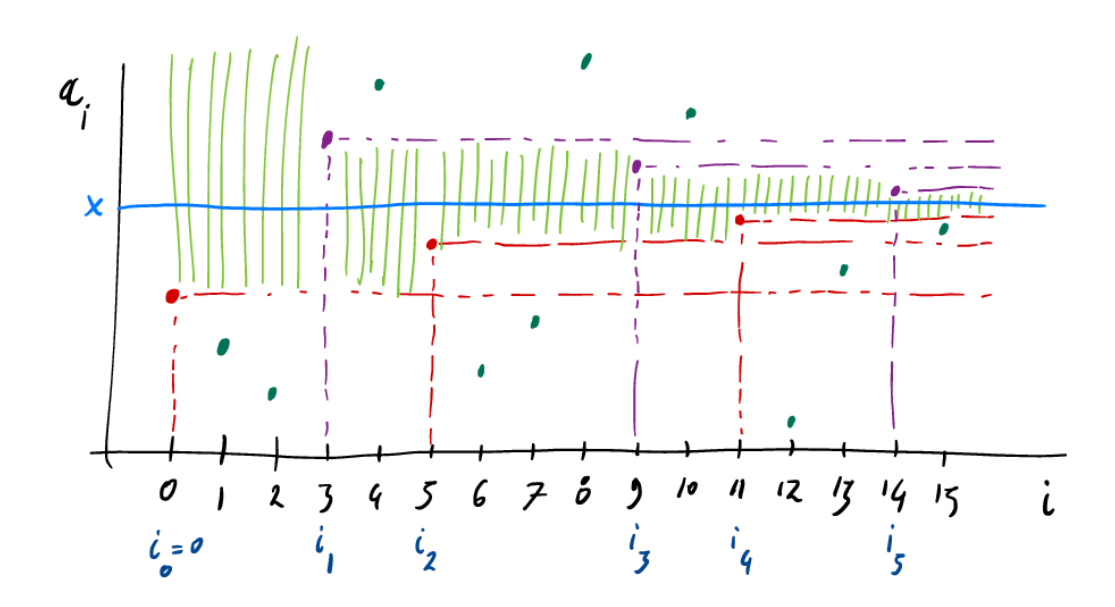
\includegraphics[width=10.5cm]{immagini/RRnum.png}
	\end{figure}

Si vede facilmente (esercizio!) che la successione $\{a_{i_{2k}}\}_k$ è crescente, $\{a_{i_{2k+1}}\}_k$ è decrescente 
e $ \lim_{k \to +\infty} a_{i_{2k}} \leq \lim_{k \to +\infty}a_{i_{2k+1}}$. Fissiamo $x$ tale che $ \lim_{k \to +\infty} a_{i_{2k}} \leq x \leq \lim_{k \to +\infty} a_{i_{2k+1}}$.
Chiaramente $x$ non è nessuno degli $a_{i_j}$, perché $a_{i_2k} < x < a_{i_{2k+1}}$. Supponiamo $x = a_n$, allora ci sarà $j$ tale che $i_j < n < i_{j+1}$, ma 
questo è assurdo perché allora $x = a_n$ è compreso fra $a_{i_{j-1}}$ e $a_{i_j}$, però $n < i_{j+1}$ contro la minimalità di quest'ultimo.

\begin{exercise}
Completare la dimostrazione nel caso $n < i$.
\end{exercise}

\begin{exercise}
Dimostrare che l'insieme di Cantor $C$ non è numerabile.
\end{exercise}
\end{proof}

\pagebreak
\subsection{Tornando agli insiemi di unicità}

\begin{theorem}
[Cantor-Lebesgue]
\label{CL}
Se $X \subseteq \RR$ è chiuso e numerabile, allora $X$ soddisfa $(\star)$, e quindi è di unicità.
\end{theorem}

La strategia di dimostrazione passa attraverso una definizione.

\begin{definition}
Dato $X \subseteq \RR$, il \vocab{derivato di Cantor-Bendixson} di $X$ è:
\[ X^{\prime} = X \setminus\{\text{punti isolati di $X$}\}
	\]
(dove $a \in X$ è un \vocab{punto di accumulazione} se $\exists \varepsilon > 0 :\, ]a - \varepsilon, a + \varepsilon[ \,\cap\, X = \{a\}$).
\end{definition}

\begin{remark}[Derivato di un chiuso soddisfa $(\star) \implies$ chiuso soddisfa $(\star)$]
Se $X$ è chiuso e $X^{\prime}$ soddisfa $(\star)$ - per cui $X'$ è di unicità per il criterio -, allora anche $X$ è di unicità.
\end{remark}

Dimostriamo questo fatto.

\begin{proof}
Occorre dimostrare che se $f : \RR \to \RR$ è continua, lineare quando ristretta agli intervalli aperti che non intersecano $X$, e non ha punti angolosi, allora $f$ è lineare, in tal modo sono soddisfatte le ipotesi del \hyperref[unicità]{Fatto 1.5} ed $X$ è di unicità.\\
Per fare ciò osserviamo che, data $f$ come sopra, se dimostriamo che quando è ristretta agli intervalli aperti che non intersecano $X'$ è lineare (e non avendo punti angolosi in generale quest'ipotesi è in automatico verificata) - essendo che quest'ultimo rispetta $(\star)$, cioè verifica le ipotesi del \hyperref[unicità]{Fatto 1.5} - allora si ottiene che $f$ è in generale lineare e quindi anche $X$ soddisfa le ipotesi del criterio.\\
Consideriamo un intervallo aperto che non interseca $X'$, $]a,b[ \,\cap\, X^{\prime} = \emptyset$, dobbiamo verificare che $f_{|\,]a,b[}$ è lineare. Ci basta dire che per ogni $\varepsilon > 0$, $f_{|[a+\varepsilon, b-\varepsilon]}$ è lineare - cioè che è lineare su ogni sottointervallo, dopodiché è banale che se vale per ogni $\varepsilon > 0$, vale in generale, e quindi $f_{|\,]a,b[}$ è lineare -.\\
Siccome per ipotesi $]a,b[ \, \cap \, X^{\prime} = \emptyset$, allora $]a,b[ \,\cap\, X \subseteq \{\text{punti isolati di $X$}\}$. Quindi l'intersezione con un sottointervallo chiuso $[a+\varepsilon, b-\varepsilon] \cap X$ è finita, se così non fosse, avrebbe che esiste nell'intersezione un punto di accumulazione 
$\alpha$ che naturalmente non può essere un punto isolato di $X\;\lightning$. Per cui $f_{|[a+\varepsilon, b-\varepsilon]}$ è lineare a tratti, e, siccome per ipotesi non ha punti angolosi (ed è continua), è lineare su tutto il sottointervallo.
\end{proof}

\begin{corollary}[Derivato $n$-esimo soddisfa $(\star) \implies$ insieme soddisfa $(\star)$]
Detto $X^{(n)}$ il derivato $n$-esimo di $X$, se per $X^{(n)}$ vale $(\star)$, per qualche $n \in \NN$, allora anche per $X$ vale $(\star)$, quindi per il \hyperref[unicità]{Fatto 1.5} è di unicità.\footnote{Il caso con $X^{(n)} = \emptyset$ scritto da Mamino nelle note è un caso particolare di questo.}
\end{corollary}

\begin{proof}
È una facile induzione su $n$, il caso $0$ è banale, mentre per il caso $n = 1$ vale l'osservazione vista sopra. Supponiamo ora che se $X^{(n-1)}$ soddisfa $(\star)$, allora 
anche $X$ soddisfa $(\star)$, e verifichiamo che se $X^{(n)}$ soddisfa $(\star)$ allora anche $X$ lo soddisfa.\\
Detto $X^{(n-1)} = Y$, allora $Y' = X^{(n)}$, dunque vale l'osservazione sopra, quindi $Y = X^{(n-1)}$ soddisfa $(\star)$ e per ipotesi induttiva anche $X$ soddisfa $(\star)$.
\end{proof}

Il guaio è che ci sono chiusi numerabili per cui $X^{(n)} \ne \emptyset$, qualunque sia $n$ - per cui non possiamo usare il corollario sopra per dedurre che sono di unicità -.

\begin{example}
Vogliamo costruire $X$ chiuso e numerabile tale che $X^{(n)} \ne \emptyset$ per ogni $n \in \NN$. Cominciamo col rivedere alcuni esempi già visti.
\end{example}

\begin{figure}[H]
		\centering
		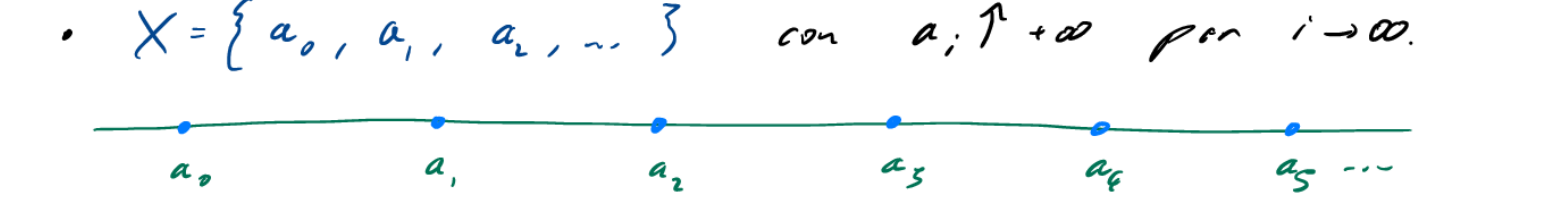
\includegraphics[scale = 0.3]{immagini/es1.png}
\end{figure}

Tutti i punti sono isolati, $X^{\prime} = \emptyset$.

\begin{figure}[H]
	\centering
	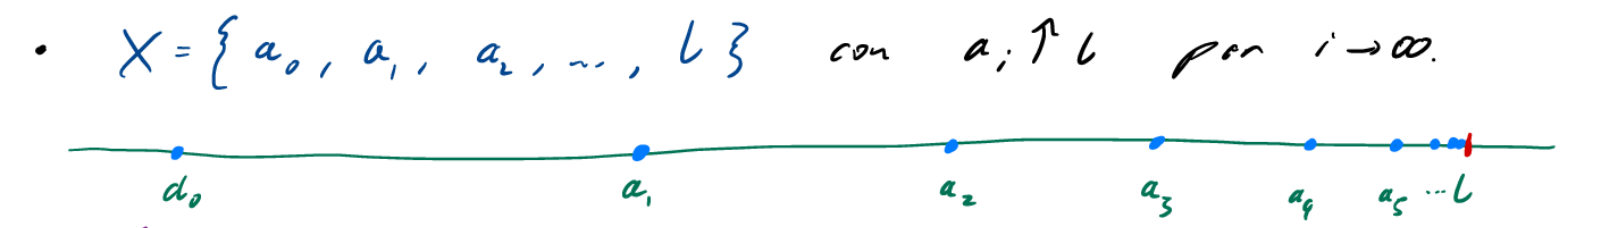
\includegraphics[scale = 0.3]{immagini/es2.png}
\end{figure}

``Successione con punto limite". Tutti i punti sono isolati salvo $l$, quindi $X^{\prime} = \{l\}$ e $X^{\prime\prime} = \emptyset$.

\begin{figure}[H]
	\centering
	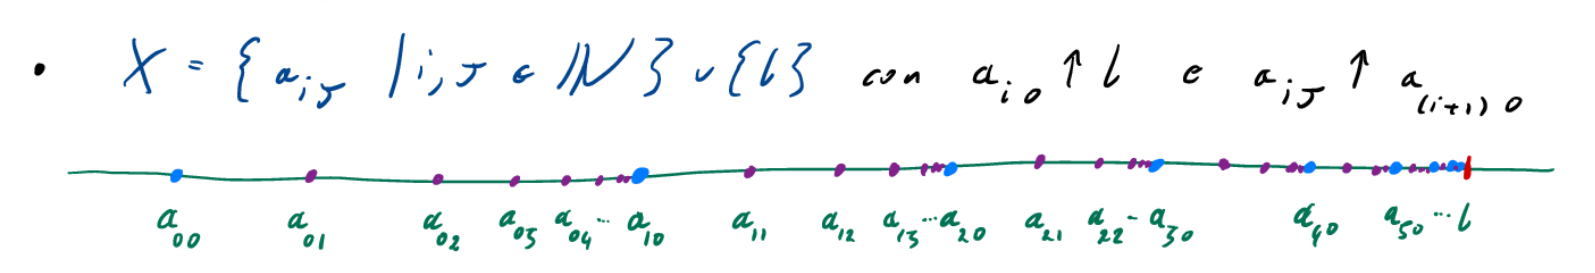
\includegraphics[scale = 0.3]{immagini/es3.png}
\end{figure}

``Successione di successioni", $X^{\prime} = \{a_{10}, a_{20}, \ldots, l\}$, $X^{\prime\prime} = \{l\}$ e $X^{\prime\prime\prime} = \emptyset$.\\
Si vede che possiamo proseguire, in qualche modo, costruendo una successione di successioni di successioni, etc. $n$ volte, $X_n$. Avremo $X_n^{(n)} \ne \emptyset$, $X_n^{(n+1)} = \emptyset$. Ora costruiamo 
$X_{\omega}$ fatto così:

\begin{figure}[H]
	\centering
	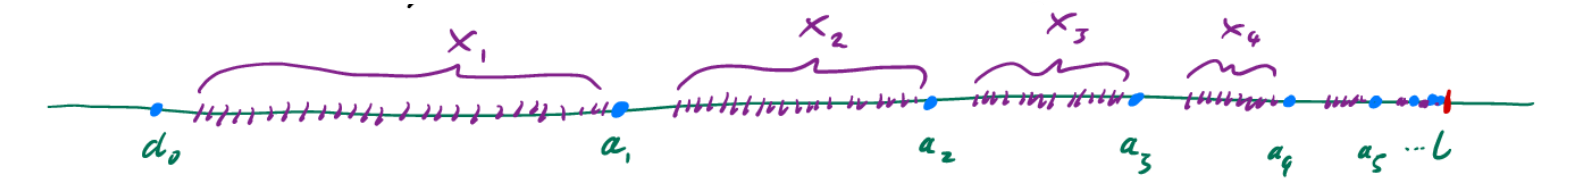
\includegraphics[scale = 0.3]{immagini/esomega.png}
\end{figure}

È chiaro che, per ogni $n$, $X_\omega^{(n)} \ne \emptyset$. D'altro canto, $X_\omega$ soddisfa il \hyperref[unicità]{Fatto 1.5}, perché $f$ deve essere lineare in ciascuno degli intervalli
$[a_n,a_{n+1}]$, perché $X_{n+1}$ soddisfa il \hyperref[unicità]{Fatto 1.5}, quindi ci si riduce al caso della successione.

\begin{exercise}
Perché $X_\omega$ è numerabile?
\end{exercise}

Ora potremmo pensare che, pazienza se $X_\omega$ non si smonta a furia di derivati, sarà un caso particolare. Però adesso, possiamo fare una successione di insiemi come $X_\omega$, chiamiamola $X_{\omega+1}$, e 
una successione di questi $X_{\omega+2}$, etc.\\
Al diavolo, serve un nuovo corollario!

\begin{corollary}
Se $X^{(n)}$ è di ``tipo $X_\omega$", allora per $X$ vale il \hyperref[unicità]{Fatto 1.5}.
\end{corollary}

Ok, questo corollario copre $X_\omega$, $X_{\omega + 1}$, $X_{\omega + 2}$, ma copre anche $X_{\omega \cdot 2}$?

\begin{figure}[H]
		\centering
		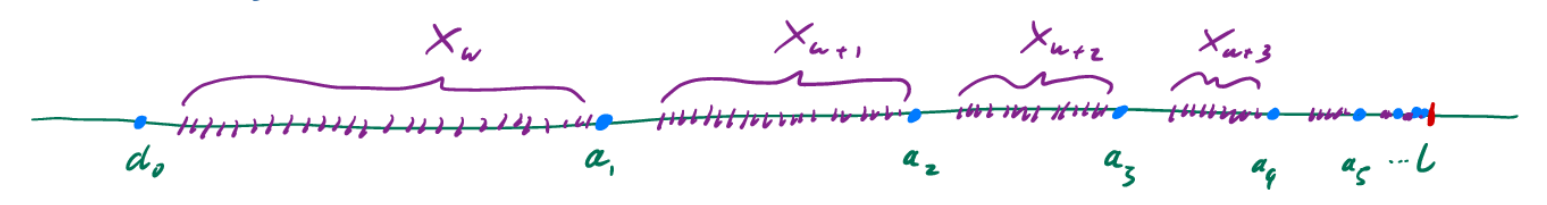
\includegraphics[scale = 0.3]{immagini/2omega.png}
\end{figure}

No: occorre un nuovo corollario.

\begin{corollary}
Se $X^{(n)}$ è di ``tipo $X_{\omega \cdot 2}$", allora per $X$ vale il \hyperref[unicità]{Fatto 1.5}.
\end{corollary}

E poi un altro per $X_{\omega \cdot 3}$, e un altro per $X_{\omega \cdot 4}$, etc.\\
E ora abbiamo finito? No, perché possiamo costruire una nuova successione con $X_{\omega},X_{\omega \cdot 2},X_{\omega \cdot 3}$, etc.\\
Se chiamiamo questa follia $X_{\omega \cdot \omega}$, ecco che si riparte a fare successioni di $X_{\omega \cdot \omega}$. Ora si sarà capito che definiremo
una serie aritmetica di queste cose, per cui potremo fare anche $\omega^\omega$, $\omega^{\omega^{\omega}}$, etc. È questa la soluzione allora?\\
No, ogni sforzo di trovare l'induzione a capo delle induzioni è vano. Se ho $X_{\omega}$, $X_{\omega^\omega}$, $X_{\omega^{\omega^{\omega}}}$, etc., allora,
ecco che faccio una successione con queste cose, la battezzo in qualche modo - ad esempio, $X_{\varepsilon_0}$ - e si riparte!\\
Per smontare ogni possibile insieme chiuso e numerabile occorre un \textbf{nuovo tipo di induzione}, l'\vocab{induzione transfinita}, che è strettamente più potente dell'induzione aritmetica.
Questa tecnica è stata sviluppata da Cantor, forse prendendo le mosse dal problema degli insiemi di unicità, e sarà uno degli argomenti centrali del corso.

\begin{exercise}[per la fine del corso]
Dimostrare il teorema di \hyperref[CL]{Cantor-Lebesgue}.
\end{exercise}

\subsection{Giochi di parole}
Descrivere un oggetto matematico non basta per crearlo. Se bastasse, si incorrerebbe in contraddizioni come queste.
\paragraph*{Paradosso di Russell}\mbox{}\\
Tipicamente le collezioni - uso questa parola perché daremo, al termine ``insieme", un senso tecnico preciso - non sono membro di se stesse: la collezione di 
tutti i numeri primi non è un numero primo. Però ci sono anche collezioni che sono membri di se stessi: per esempio la collezione di tutte le collezioni. Consideriamo:
\[ N = \{\text{collezioni $X$}\, | X \not\in X \}
	\]
la collezione delle collezioni che non sono membri di se stessi - la $N$ sta per collezioni normali. Quindi ci chiediamo se $N \in N$ oppure no? $N \in N$ se e solo se per definizione $N \not \in N$, che è assurdo.\\
Il paradosso di Russell ci dice che, del principio di collezione - ossia l'idea che data una proprietà ben definita $P$ si possa costruire la collezione $\{X | P(X)\}$ - non ci si può fidare.

\paragraph*{Paradosso di Berry}\mbox{}\\
L'italiano annovera un numero finito di parole, è quindi possibile formare solo un numero finito di frasi di meno di cento parole. Alcune di queste descrivono un numero naturale, altre no. Comunque, solo un numero 
finito di numeri naturali può essere descritto con meno di cento parole. Per il principio del minimo, esiste:
\begin{align*}
	h = \text{``il più piccolo numero naturale che l'italiano non può} \\ 
 \text{descrivere con meno di cento parole"}
\end{align*}
Il guaio chiaramente, è che lo abbiamo appena descritto con sedici parole.\\
Quindi non ci si può fidare troppo neppure dell'italiano, o meglio, non è possibile descrivere precisamente cosa sia una descrizione precisa.\\
In conclusione, occorre fissare un linguaggio formale in cui si esprimano le proposizioni della teoria degli insiemi, e occorre fissare un sistema di assiomi, espressi in questo linguaggio, che 
dicano quali costruzioni sono lecite: quali insiemi esistono. Il ruolo della teoria degli insiemi è, poi, di fondare l'edificio della matematica. L'ambizione, quindi, è che il linguaggio e gli assiomi della teoria degli insiemi, 
siano in realtà, il linguaggio e gli assiomi della matematica.

\subsection{Scopi del corso}
Questo corso persegue due obiettivi:
\begin{enumerate}[(1)]
	\item Studiare i \textbf{fondamenti della matematica}, nella forma più comunemente accettata nel XX secolo e fino ad ora, la teoria degli insiemi di 
	\href{https://it.wikipedia.org/wiki/Ernst_Zermelo}{\textcolor{purple}{Zermelo}}-\href{https://it.wikipedia.org/wiki/Adolf_Abraham_Halevi_Fraenkel}{\textcolor{purple}{Fraenkel}} con l'assioma della scelta (ZFC).
	\item Studiare tecniche e strumenti che sono stati sviluppati grazie alla teoria degli insiemi, per esempio: la teoria delle cardinalità, la teoria dei numeri ordinali, l'induzione e la ricorsione transfinita.
\end{enumerate}

In questo corso non ci occupiamo dei modelli della teoria degli insiemi. Mi spiego. Per esempio, in teoria dei gruppi si assiomatizza cosa sia un gruppo, e poi si studia come possano essere fatti i diversi gruppi. In 
teoria degli insiemi si assiomatizza l'universo di tutti gli insiemi, però, per il teorema di incompletezza di \href{https://it.wikipedia.org/wiki/Kurt_G%C3%B6del}{\textcolor{purple}{Gödel}}, questa assiomatizzazione non 
può essere completa. Quindi esistono tanti universi insiemistici possibili. Indagare queste possibilità - i modelli della teoria degli insiemi - è argomento di corsi più avanzati.
